\documentclass[11pt,aspectratio=169]{beamer}

% Encodage et langue
\usepackage[utf8]{inputenc}
\usepackage[T1]{fontenc}
\usepackage[french]{babel}

% Typographie et mise en page
\usepackage{lmodern}
\usepackage{microtype}
\usepackage{ragged2e}

% Figures, tableaux et mathématiques
\usepackage{graphicx}
\usepackage{booktabs}
\usepackage{array}
\usepackage{amsmath,amssymb}
\usepackage{tikz}
\usetikzlibrary{arrows.meta,positioning,calc,fit}

\graphicspath{{figures/}{./}{memoire/figures/}{memoire/}}

% -----------------------------------------------------------------------------
% Identité visuelle
% -----------------------------------------------------------------------------
\definecolor{Ink}{HTML}{243238}
\definecolor{DeepTeal}{HTML}{174D59}
\definecolor{Teal}{HTML}{1B8594}
\definecolor{Blue}{HTML}{3B6195}
\definecolor{Coral}{HTML}{D96C4F}
\definecolor{SoftGray}{HTML}{F1F4F5}
\definecolor{MidGray}{HTML}{68777D}
\definecolor{RuleGray}{HTML}{D7DEE1}

\setbeamercolor{normal text}{fg=Ink,bg=white}
\setbeamercolor{structure}{fg=Teal}
\setbeamercolor{frametitle}{fg=Ink,bg=white}
\setbeamercolor{title}{fg=white}
\setbeamercolor{subtitle}{fg=white}
\setbeamercolor{block title}{fg=white,bg=DeepTeal}
\setbeamercolor{block body}{fg=Ink,bg=SoftGray}
\setbeamercolor{block title alerted}{fg=white,bg=Coral}
\setbeamercolor{block body alerted}{fg=Ink,bg=Coral!9}
\setbeamercolor{author in head/foot}{fg=white,bg=DeepTeal}
\setbeamercolor{section in head/foot}{fg=white,bg=Teal}
\setbeamercolor{page number in head/foot}{fg=white,bg=Ink}

\setbeamerfont{title}{size=\LARGE,series=\bfseries}
\setbeamerfont{subtitle}{size=\large}
\setbeamerfont{frametitle}{size=\Large,series=\bfseries}
\setbeamerfont{block title}{series=\bfseries}
\setbeamerfont{footline}{size=\scriptsize}

\setbeamertemplate{navigation symbols}{}
\setbeamertemplate{itemize item}{\color{Teal}$\blacktriangleright$}
\setbeamertemplate{itemize subitem}{\color{Coral}$\bullet$}
\setbeamertemplate{enumerate item}{%
  \tikz[baseline=(n.base)]\node[circle,fill=Teal,text=white,
    inner sep=1.2pt,font=\scriptsize\bfseries] (n) {\insertenumlabel};}
\setbeamertemplate{blocks}[rounded][shadow=false]
\setbeamersize{text margin left=0.6cm,text margin right=0.6cm}

\setbeamertemplate{frametitle}{%
  \vspace{0.18cm}%
  \begin{beamercolorbox}[wd=\paperwidth,ht=0.68cm,dp=0.08cm,leftskip=0.6cm]{frametitle}
    \usebeamerfont{frametitle}\insertframetitle
  \end{beamercolorbox}%
  \vspace{-0.06cm}%
  {\hspace{0.6cm}\color{Teal}\rule{1.25cm}{1.5pt}%
  \color{RuleGray}\rule{\dimexpr\paperwidth-2.45cm\relax}{0.45pt}}%
  \vspace{0.08cm}%
}

\setbeamertemplate{footline}{%
  \leavevmode%
  \hbox{%
    \begin{beamercolorbox}[wd=.25\paperwidth,ht=2.6ex,dp=1.1ex,leftskip=.5cm]{author in head/foot}
      \usebeamerfont{footline}\insertshortauthor
    \end{beamercolorbox}%
    \begin{beamercolorbox}[wd=.60\paperwidth,ht=2.6ex,dp=1.1ex,leftskip=.4cm]{section in head/foot}
      \usebeamerfont{footline}\insertsectionhead
    \end{beamercolorbox}%
    \begin{beamercolorbox}[wd=.15\paperwidth,ht=2.6ex,dp=1.1ex,center]{page number in head/foot}
      \usebeamerfont{footline}\insertframenumber/\inserttotalframenumber
    \end{beamercolorbox}%
  }%
}

\newcommand{\source}[1]{%
  \par\vspace{0.08cm}{\scriptsize\color{MidGray}#1}%
}

\newcommand{\takeaway}[1]{%
  \begin{beamercolorbox}[wd=\linewidth,sep=0.55em,rounded=true]{block body}
    \centering\bfseries\color{DeepTeal}#1
  \end{beamercolorbox}%
}

\newcommand{\metric}[3]{%
  \begin{beamercolorbox}[wd=\linewidth,sep=0.45em,rounded=true]{block body}
    {\scriptsize\color{MidGray}#1}\par
    {\large\bfseries\color{#3}#2}
  \end{beamercolorbox}%
}

% -----------------------------------------------------------------------------
% Informations de la soutenance
% -----------------------------------------------------------------------------
\title[Vectorisation raster-vers-SVG]{Vectorisation automatique d'images matricielles par Deep Learning}
\subtitle{Projet de fin d'études}
\author[BITAM \& AITHAMOUDI]{Amir BITAM \and Zakaria AITHAMOUDI}
\institute{Higher Institute of Sciences}
\date{Année universitaire 2025--2026}

\hypersetup{
  pdftitle={Vectorisation automatique d'images matricielles par Deep Learning},
  pdfauthor={Amir BITAM et Zakaria AITHAMOUDI}
}

\begin{document}

% -----------------------------------------------------------------------------
% Titre
% -----------------------------------------------------------------------------
\begin{frame}[plain]
  \begin{tikzpicture}[remember picture,overlay]
    \fill[Ink] (current page.south west) rectangle (current page.north east);
    \fill[Teal] (current page.south west) rectangle
      ([xshift=0.16cm]current page.north west);
    \fill[Coral] ([yshift=-0.16cm]current page.north west) rectangle
      ([yshift=-0.23cm]current page.north east);
    \node[anchor=north east,fill=white,rounded corners=2pt,inner sep=0.15cm]
      at ([xshift=-0.75cm,yshift=-0.75cm]current page.north east)
      {
\includegraphics[height=2.15cm]{his_logo.png}};
  \end{tikzpicture}

  \vspace*{0.9cm}
  \begin{minipage}{0.76\paperwidth}
    {\color{Coral}\large\bfseries PROJET DE FIN D'ÉTUDES}\par\vspace{0.35cm}
    {\color{white}\fontsize{25}{29}\selectfont\bfseries
      Vectorisation automatique\\
      d'images matricielles\\
      par Deep Learning}\par\vspace{0.45cm}
    {\color{white!76}\large De l'image raster aux chemins SVG éditables}
  \end{minipage}

  \vfill
  \begin{columns}[T,onlytextwidth]
    \begin{column}{0.48\textwidth}
      {\color{white!68}\small Présenté par}\par
      {\color{white}\large\bfseries Amir BITAM}\par
      {\color{white}\large\bfseries Zakaria AITHAMOUDI}
    \end{column}
    \begin{column}{0.48\textwidth}
      \raggedleft
      {\color{white!68}\small Encadré par}\par
      {\color{white}\large\bfseries Hamza ABDELLAHOUM}\par\vspace{0.12cm}
      {\color{white!68}\small Higher Institute of Sciences · 2025--2026}
    \end{column}
  \end{columns}
  \vspace{0.45cm}
\end{frame}

% -----------------------------------------------------------------------------
% Plan
% -----------------------------------------------------------------------------
\begin{frame}{Plan de la présentation}
  \vspace{0.2cm}
  \tableofcontents[hideallsubsections]

  \vfill
  \takeaway{Fil conducteur : représenter fidèlement une image avec des primitives rapides à produire et réellement éditables.}
\end{frame}

% -----------------------------------------------------------------------------
\section{Contexte et état de l'art}
% -----------------------------------------------------------------------------

\begin{frame}{Contexte et problématique}
  \begin{columns}[T,onlytextwidth]
    \begin{column}{0.59\textwidth}
      \centering
      
\includegraphics[width=\linewidth]{figure_raster_vector.png}
      \source{Image matricielle à gauche, représentation vectorielle à droite.}
    \end{column}
    \begin{column}{0.37\textwidth}
      \begin{block}{Image matricielle}
        Grille finie de pixels, adaptée aux photographies mais dépendante de la résolution.
      \end{block}
      \begin{block}{Image vectorielle}
        Primitives géométriques redimensionnables, structurées et éditables.
      \end{block}
    \end{column}
  \end{columns}

  \vspace{0.2cm}
  \begin{alertblock}{Question de recherche}
    Comment retrouver automatiquement les régions, les contours et les couleurs d'une image naturelle avec un SVG fidèle, rapide à générer et de complexité maîtrisée ?
  \end{alertblock}
\end{frame}

\begin{frame}{Des approches classiques à la prédiction directe}
  \centering
  \scriptsize
  \renewcommand{\arraystretch}{1.25}
  \begin{tabular}{>{\bfseries}p{2.25cm}p{3.15cm}p{3.45cm}p{4.65cm}}
    \toprule
    Approche & Principe & Atout principal & Limite principale \\
    \midrule
    Potrace & Tracé algorithmique & Rapide, sans apprentissage & Principalement adapté aux images binaires \\
    LIVE & Optimisation par image & SVG compact et structuré & Plusieurs milliers d'itérations par entrée \\
    Im2Vec & Décodeur de formes latentes & Pas de supervision SVG & Généralisation limitée hors du domaine entraîné \\
    SuperSVG & Superpixels et \textit{coarse-to-fine} & Forte fidélité & Pipeline plus complexe et nombreux chemins \\
    Notre approche & DINOv3 et requêtes de chemins & Prédiction directe en une étape & Nombre fixe de primitives par région \\
    \bottomrule
  \end{tabular}

  \vfill
  \takeaway{Notre positionnement : conserver la décomposition locale de SuperSVG, avec un décodeur unique fondé sur l'attention.}
  \source{Références principales : Selinger (2003), Reddy et al. (2021), Ma et al. (2022), Hu et al. (2024).}
\end{frame}

% -----------------------------------------------------------------------------
\section{Approche proposée}
% -----------------------------------------------------------------------------

\begin{frame}{Vue d'ensemble de la méthode}
  \centering
  \resizebox{\textwidth}{!}{%
  \begin{tikzpicture}[
      node distance=0.48cm,
      box/.style={draw=RuleGray,rounded corners=2pt,align=center,
        minimum height=1.05cm,text width=1.85cm,inner sep=4pt,font=\small},
      data/.style={box,fill=SoftGray},
      process/.style={box,fill=Teal!10,draw=Teal!65},
      learned/.style={box,fill=Blue!10,draw=Blue!70},
      result/.style={box,fill=Coral!10,draw=Coral!75},
      arrow/.style={-{Latex[length=2.4mm]},thick,draw=Ink!78}
    ]
    \node[data] (image) {Image RGB\\matricielle};
    \node[process,right=of image] (slic) {Segmentation\\SLIC};
    \node[process,right=of slic] (crop) {Recadrage\\et masque};
    \node[learned,right=of crop] (dino) {Backbone\\DINOv3};
    \node[learned,right=of dino] (attn) {Cross-attention\\Self-attention};
    \node[result,right=of attn] (paths) {$P$ chemins\\$P\times27$ paramètres};
    \node[result,right=of paths] (svg) {Assemblage\\SVG};

    \node[process,below=1.0cm of paths] (render) {Rendu\\DiffVG};
    \node[result,left=of render] (loss) {Pertes de\\reconstruction};

    \draw[arrow] (image)--(slic);
    \draw[arrow] (slic)--(crop);
    \draw[arrow] (crop)--(dino);
    \draw[arrow] (dino)--(attn);
    \draw[arrow] (attn)--(paths);
    \draw[arrow] (paths)--(svg);
    \draw[arrow] (paths)--(render);
    \draw[arrow] (render)--(loss);
    \draw[arrow,Coral] (loss.west)-| ($(dino.south)+(0,-0.12)$);

    \node[font=\scriptsize\bfseries,text=Coral,below=0.08cm of loss]
      {Branche d'entraînement};
    \node[font=\scriptsize\bfseries,text=Teal,above=0.08cm of svg]
      {Inférence directe};
  \end{tikzpicture}%
  }

  \vspace{0.5cm}
  \begin{columns}[T,onlytextwidth]
    \begin{column}{0.32\textwidth}
      \metric{Entrée locale}{$3\times224\times224$}{Teal}
    \end{column}
    \begin{column}{0.32\textwidth}
      \metric{Sortie par chemin}{$12$ points $+$ RGB}{Blue}
    \end{column}
    \begin{column}{0.32\textwidth}
      \metric{Supervision}{Images matricielles seules}{Coral}
    \end{column}
  \end{columns}
\end{frame}

\begin{frame}{Préparation par superpixels SLIC}
  \centering
  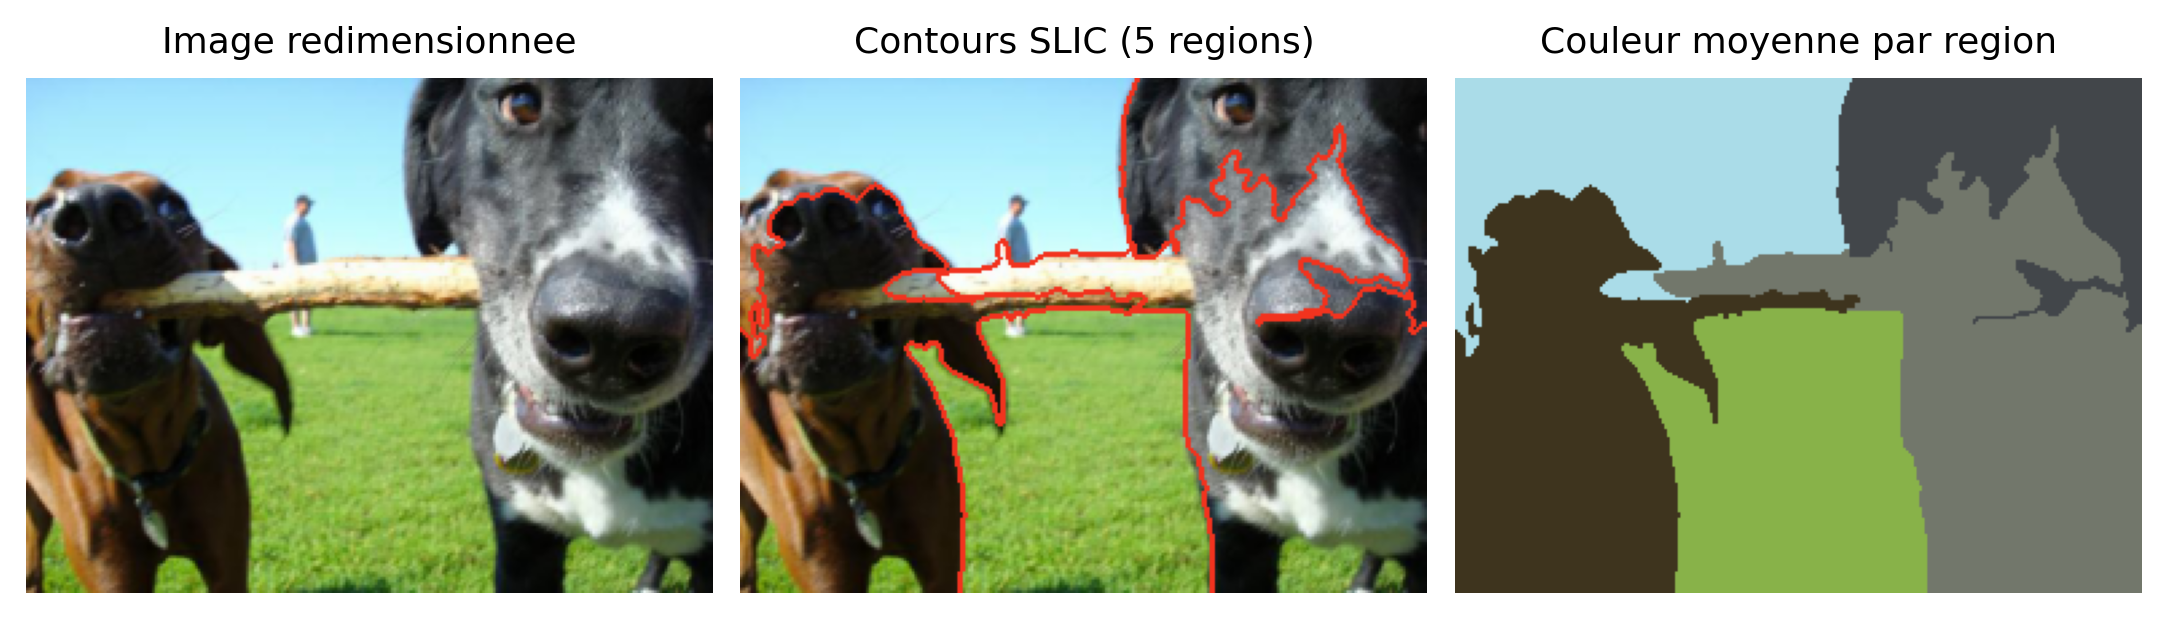
\includegraphics[width=\textwidth]{ch3_segmentation_slic.png}

  \vspace{0.25cm}
  \begin{columns}[T,onlytextwidth]
    \begin{column}{0.32\textwidth}
      \begin{block}{1. Segmenter}
        Regrouper les pixels proches en couleur et dans l'espace.
      \end{block}
    \end{column}
    \begin{column}{0.32\textwidth}
      \begin{block}{2. Recadrer}
        Extraire la boîte englobante et conserver un masque binaire.
      \end{block}
    \end{column}
    \begin{column}{0.32\textwidth}
      \begin{block}{3. Normaliser}
        Redimensionner chaque région en $224\times224$ avant l'encodage.
      \end{block}
    \end{column}
  \end{columns}

  \source{SLIC demandé avec 16 régions, compacité 10 et $\sigma=1$ dans les expériences principales.}
\end{frame}

\begin{frame}{Architecture de prédiction des chemins}
  \centering
  \resizebox{0.97\textwidth}{!}{%
  \begin{tikzpicture}[
      node distance=0.55cm,
      box/.style={draw=RuleGray,rounded corners=2pt,align=center,
        minimum height=1.0cm,text width=2.1cm,inner sep=4pt,font=\small},
      visual/.style={box,fill=Blue!10,draw=Blue!70},
      query/.style={box,fill=Coral!10,draw=Coral!75},
      op/.style={box,fill=Teal!10,draw=Teal!70},
      arrow/.style={-{Latex[length=2.5mm]},thick,draw=Ink!78}
    ]
    \node[visual] (input) {Région\\$3\times224\times224$};
    \node[visual,right=of input] (dino) {DINOv3--ViT\\patch $16\times16$};
    \node[visual,right=of dino] (tokens) {$196$ tokens\\visuels $F$};
    \node[op,right=1.0cm of tokens] (cross) {Cross-attention\\$Q$ chemins, $K,V$ image};
    \node[op,right=of cross] (self) {Self-attention\\entre chemins};
    \node[query,right=of self] (head) {LayerNorm\\projection, sigmoïde};
    \node[query,right=of head] (out) {$Z\in[0,1]^{P\times27}$};
    \node[query,below=0.9cm of cross] (queries) {$P$ requêtes\\apprenables};

    \draw[arrow] (input)--(dino);
    \draw[arrow] (dino)--(tokens);
    \draw[arrow] (tokens)--node[above,font=\scriptsize]{$K,V$}(cross);
    \draw[arrow] (queries)--node[right,font=\scriptsize]{$Q$}(cross);
    \draw[arrow] (cross)--(self);
    \draw[arrow] (self)--(head);
    \draw[arrow] (head)--(out);

    \node[draw=Coral,dashed,rounded corners=2pt,fit=(dino)(tokens),
      label={[font=\scriptsize\bfseries,text=Coral]above:backbone ajusté pendant l'entraînement}] {};
  \end{tikzpicture}%
  }

  \vspace{0.45cm}
  \begin{columns}[T,onlytextwidth]
    \begin{column}{0.31\textwidth}
      \metric{Backbone}{ViT-S/16 DINOv3}{Blue}
    \end{column}
    \begin{column}{0.31\textwidth}
      \metric{Attention}{8 têtes demandées}{Teal}
    \end{column}
    \begin{column}{0.34\textwidth}
      \metric{Version finale}{$P=128$ chemins par région}{Coral}
    \end{column}
  \end{columns}

  \source{DINOv3 fournit les caractéristiques denses; les tokens préfixes sont retirés avant le décodeur.}
\end{frame}

\begin{frame}{Représentation d'un chemin SVG}
  \begin{columns}[T,onlytextwidth]
    \begin{column}{0.57\textwidth}
      \centering
      \resizebox{0.95\linewidth}{!}{%
      \begin{tikzpicture}[
          anchorpoint/.style={circle,fill=Ink,inner sep=2.4pt},
          controlpoint/.style={circle,draw=Ink,fill=white,inner sep=2.0pt}]
        \coordinate (p0) at (0,0);
        \coordinate (p1) at (-0.8,1.2);
        \coordinate (p2) at (0.45,2.45);
        \coordinate (p3) at (2.0,2.15);
        \coordinate (p4) at (3.15,2.05);
        \coordinate (p5) at (4.25,1.2);
        \coordinate (p6) at (4.0,0.0);
        \coordinate (p7) at (3.8,-1.1);
        \coordinate (p8) at (2.7,-1.75);
        \coordinate (p9) at (1.55,-1.45);
        \coordinate (p10) at (0.45,-1.35);
        \coordinate (p11) at (-0.75,-0.75);

        \draw[densely dashed,MidGray] (p0)--(p1)--(p2)--(p3);
        \draw[densely dashed,MidGray] (p3)--(p4)--(p5)--(p6);
        \draw[densely dashed,MidGray] (p6)--(p7)--(p8)--(p9);
        \draw[densely dashed,MidGray] (p9)--(p10)--(p11)--(p0);
        \fill[Teal!14]
          (p0) .. controls (p1) and (p2) .. (p3)
               .. controls (p4) and (p5) .. (p6)
               .. controls (p7) and (p8) .. (p9)
               .. controls (p10) and (p11) .. (p0);
        \draw[very thick,Teal]
          (p0) .. controls (p1) and (p2) .. (p3)
               .. controls (p4) and (p5) .. (p6)
               .. controls (p7) and (p8) .. (p9)
               .. controls (p10) and (p11) .. (p0);

        \node[anchorpoint,label={[font=\scriptsize]below left:$P_0$}] at (p0) {};
        \node[controlpoint,label={[font=\scriptsize]left:$P_1$}] at (p1) {};
        \node[controlpoint,label={[font=\scriptsize]above:$P_2$}] at (p2) {};
        \node[anchorpoint,label={[font=\scriptsize]above:$P_3$}] at (p3) {};
        \node[controlpoint,label={[font=\scriptsize]above:$P_4$}] at (p4) {};
        \node[controlpoint,label={[font=\scriptsize]right:$P_5$}] at (p5) {};
        \node[anchorpoint,label={[font=\scriptsize]right:$P_6$}] at (p6) {};
        \node[controlpoint,label={[font=\scriptsize]right:$P_7$}] at (p7) {};
        \node[controlpoint,label={[font=\scriptsize]below:$P_8$}] at (p8) {};
        \node[anchorpoint,label={[font=\scriptsize]below:$P_9$}] at (p9) {};
        \node[controlpoint,label={[font=\scriptsize]below:$P_{10}$}] at (p10) {};
        \node[controlpoint,label={[font=\scriptsize]left:$P_{11}$}] at (p11) {};
      \end{tikzpicture}%
      }
      \source{Points pleins : ancrages; points blancs : contrôles.}
    \end{column}
    \begin{column}{0.39\textwidth}
      \begin{block}{27 paramètres prédits}
        \[
          z_p=(x_0,y_0,\ldots,x_{11},y_{11},r,g,b)
        \]
      \end{block}

      \begin{itemize}
        \item 12 points normalisés;
        \item 4 segments de Bézier cubiques;
        \item chemin fermé et opaque;
        \item couleur de remplissage RGB;
        \item aucun contour séparé.
      \end{itemize}

      \vspace{0.15cm}
      {\scriptsize
      \[
        \mathcal B(t)=(1-t)^3A+3(1-t)^2tC_1
        +3(1-t)t^2C_2+t^3B
      \]}
    \end{column}
  \end{columns}
\end{frame}

\begin{frame}{Apprentissage sans SVG de référence}
  \centering
  \resizebox{0.89\textwidth}{!}{%
  \begin{tikzpicture}[
      node distance=0.7cm,
      box/.style={draw=RuleGray,rounded corners=2pt,align=center,
        minimum height=0.95cm,text width=2.25cm,inner sep=4pt,font=\small},
      arrow/.style={-{Latex[length=2.5mm]},thick,draw=Ink!78}
    ]
    \node[box,fill=Blue!10,draw=Blue!70] (model) {DINOv3 et\\décodeur};
    \node[box,fill=Coral!10,draw=Coral!75,right=of model] (paths) {Chemins\\prédits};
    \node[box,fill=Teal!10,draw=Teal!70,right=of paths] (render) {Rasterisation\\DiffVG};
    \node[box,fill=SoftGray,right=of render] (image) {Rendu $\widehat{Y}$\\et alpha $\widehat{A}$};
    \node[box,fill=Coral!10,draw=Coral!75,right=of image] (loss) {$\mathcal L_{\mathrm{rec}}$\\$+\lambda\mathcal L_{\mathrm{ext}}$};
    \draw[arrow] (model)--(paths);
    \draw[arrow] (paths)--(render);
    \draw[arrow] (render)--(image);
    \draw[arrow] (image)--(loss);
    \draw[arrow,Coral] (loss.south) -- ++(0,-0.55) -| (model.south);
    \node[font=\scriptsize,text=Coral,below=0.55cm of image] {Rétropropagation jusqu'au backbone};
  \end{tikzpicture}%
  }

  \vspace{0.25cm}
  \begin{columns}[T,onlytextwidth]
    \begin{column}{0.49\textwidth}
      \begin{block}{Fonction objective}
        \[
          \mathcal L=\mathcal L_{\mathrm{rec}}
          +\lambda_{\mathrm{masque}}\mathcal L_{\mathrm{ext}}
        \]
        \begin{itemize}\small
          \item MSE normalisée dans le superpixel;
          \item pénalité sur l'opacité hors du masque dilaté;
          \item $\lambda_{\mathrm{masque}}: 0{,}05\rightarrow0{,}01$.
        \end{itemize}
      \end{block}
    \end{column}
    \begin{column}{0.47\textwidth}
      \begin{block}{Configuration finale}
        \scriptsize
        \begin{tabular}{@{}ll@{}}
          Données & $10\,000$ images ImageNet \\
          Chemins & $128$ par superpixel \\
          Entraînement & $20$ époques, lots de $16$ \\
          Optimiseur & AdamW, $10^{-4}$ \\
          Ordonnancement & $4$ époques de \textit{warm-up} \\
          Calcul & Précision mixte sur GPU \\
        \end{tabular}
      \end{block}
    \end{column}
  \end{columns}
\end{frame}

% -----------------------------------------------------------------------------
\section{Protocole expérimental}
% -----------------------------------------------------------------------------

\begin{frame}{Protocole d'évaluation}
  \begin{columns}[T,onlytextwidth]
    \begin{column}{0.31\textwidth}
      \begin{block}{Environnement}
        \begin{itemize}\small
          \item Windows 11;
          \item Ryzen 7 7800X3D;
          \item RTX 4070 SUPER, 12 Go;
          \item PyTorch 2.5.1 et CUDA 12.4;
          \item DiffVG avec CUDA.
        \end{itemize}
      \end{block}
    \end{column}
    \begin{column}{0.32\textwidth}
      \begin{block}{Jeux évalués}
        \begin{itemize}\small
          \item 12 images ImageNet non vues;
          \item 4 images communes aux références;
          \item côté maximal interne : $256$ pixels;
          \item entrées externes : $256\times256$;
          \item même rasteriseur pydiffvg.
        \end{itemize}
      \end{block}
    \end{column}
    \begin{column}{0.33\textwidth}
      \begin{block}{Critères}
        \begin{itemize}\small
          \item MSE $\downarrow$ et PSNR $\uparrow$;
          \item SSIM $\uparrow$ et LPIPS $\downarrow$;
          \item temps de vectorisation;
          \item chemins et segments;
          \item taille du fichier SVG.
        \end{itemize}
      \end{block}
    \end{column}
  \end{columns}

  \vspace{0.35cm}
  \begin{alertblock}{Précaution d'interprétation}
    Les configurations disponibles n'ont ni le même budget d'entraînement ni le même budget vectoriel. Les résultats décrivent les systèmes complets dans notre environnement, sans établir un classement général.
  \end{alertblock}
\end{frame}

\begin{frame}{Validation et évolution de l'apprentissage}
  \begin{columns}[T,onlytextwidth]
    \begin{column}{0.68\textwidth}
      \centering
      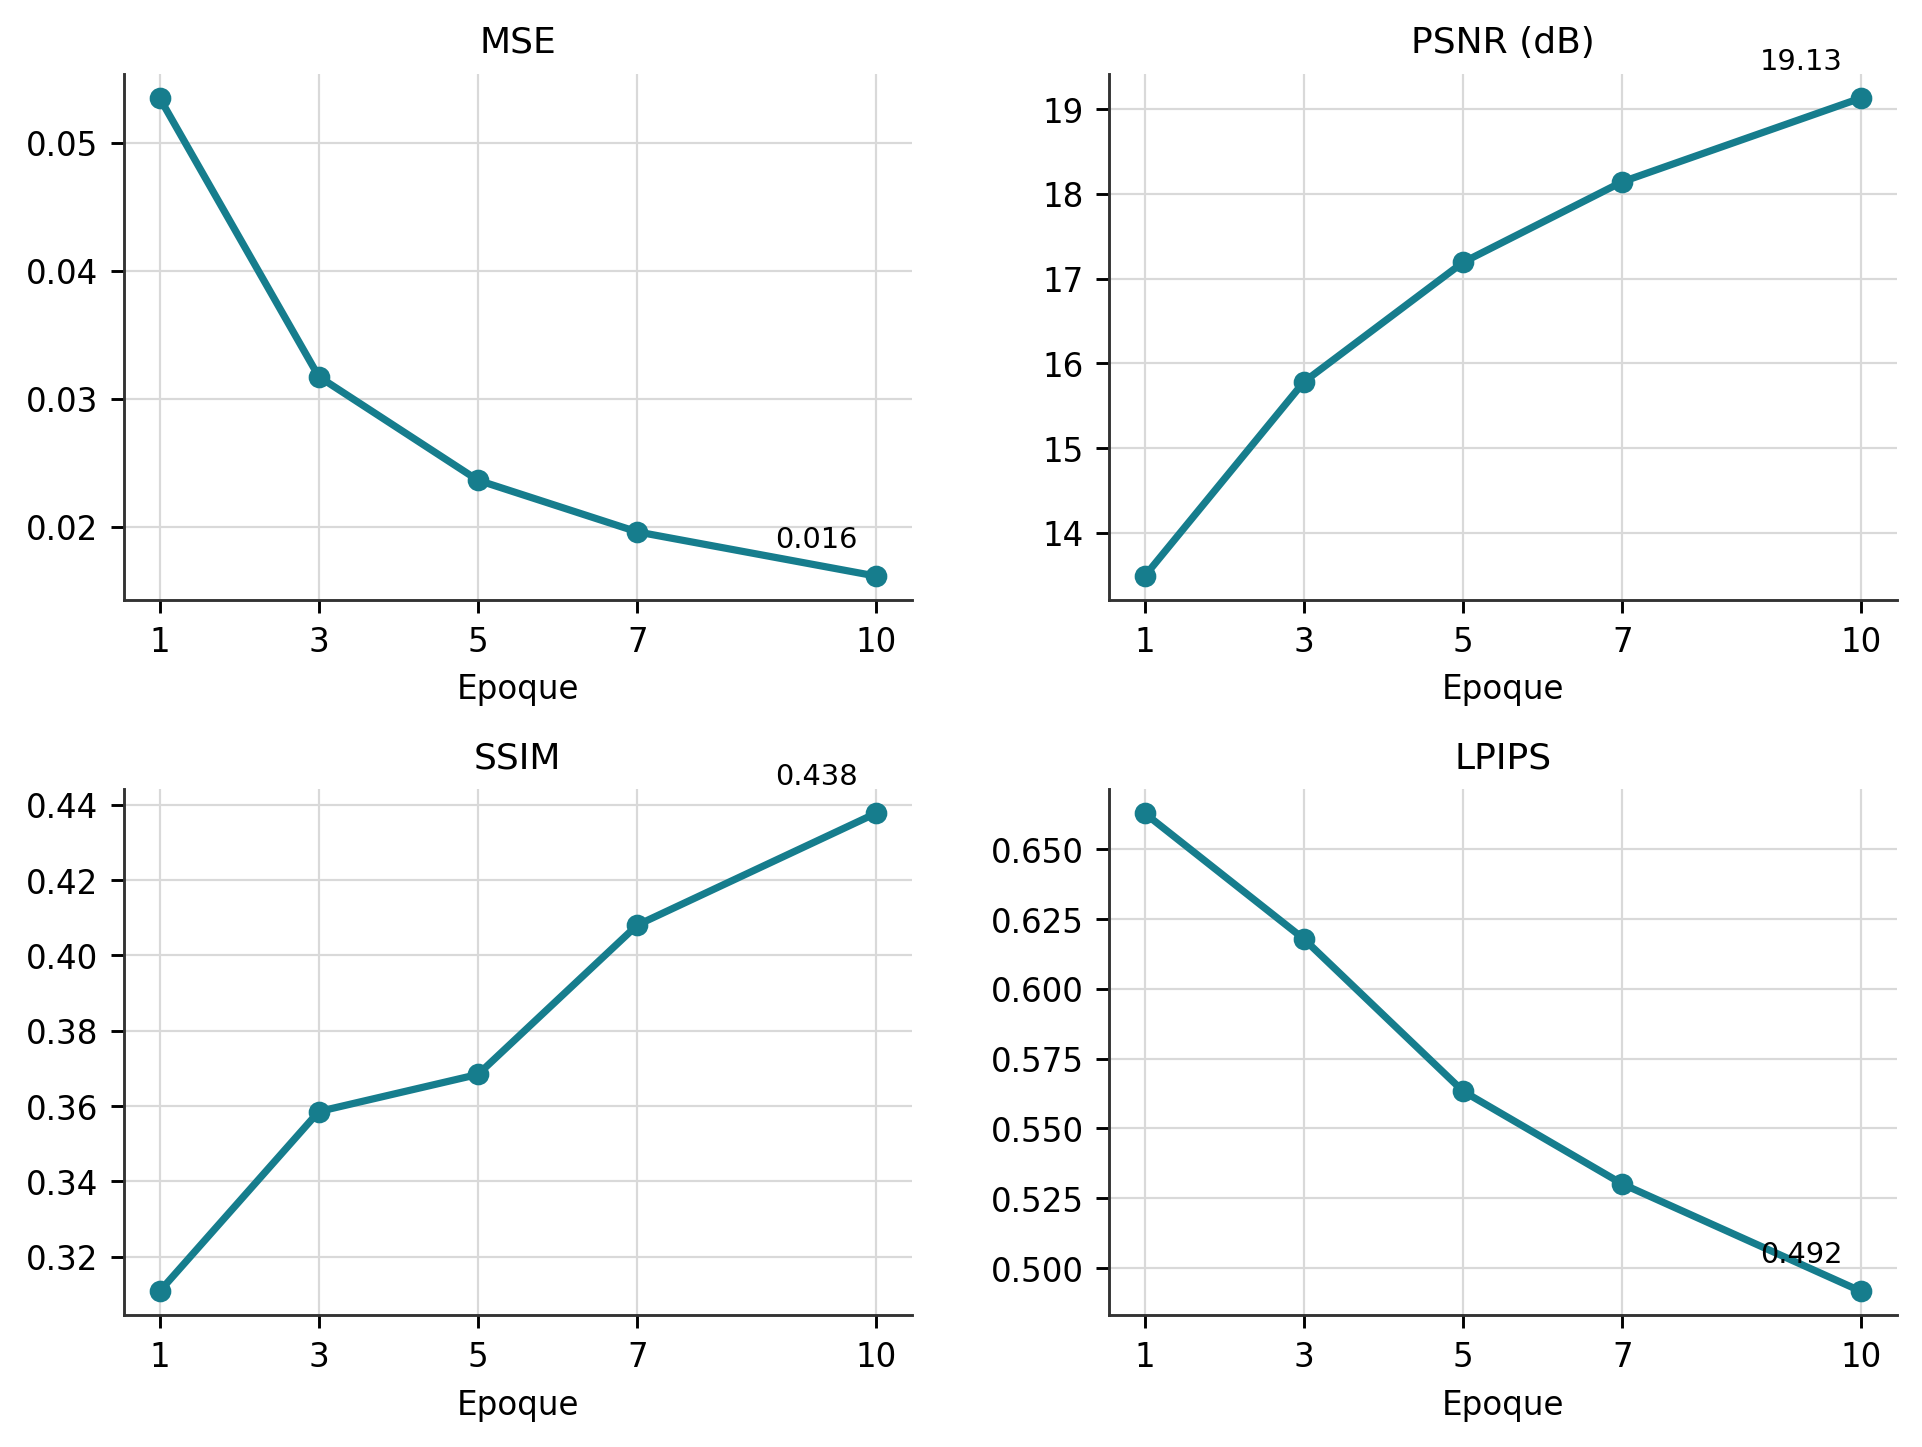
\includegraphics[width=\linewidth,height=6.2cm,keepaspectratio]{ch3_progression_entrainement.png}
    \end{column}
    \begin{column}{0.28\textwidth}
      \metric{MSE}{$0{,}05351\rightarrow0{,}01615$}{Teal}
      \vspace{0.13cm}
      \metric{PSNR}{$+5{,}64$ dB}{Blue}
      \vspace{0.13cm}
      \metric{SSIM}{$+0{,}127$}{Teal}
      \vspace{0.13cm}
      \metric{LPIPS}{$-0{,}171$}{Coral}
      \vspace{0.2cm}
      {\scriptsize\bfseries\color{DeepTeal}Contrôles techniques}\par
      {\scriptsize Gradients finis à travers DiffVG; $24/24$ SVG valides et rechargeables.}
    \end{column}
  \end{columns}
  \source{Configuration à 32 chemins évaluée aux époques 1, 3, 5, 7 et 10.}
\end{frame}

% -----------------------------------------------------------------------------
\section{Résultats}
% -----------------------------------------------------------------------------

\begin{frame}{Étude interne : 32 contre 128 chemins}
  \begin{columns}[T,onlytextwidth]
    \begin{column}{0.67\textwidth}
      \centering
      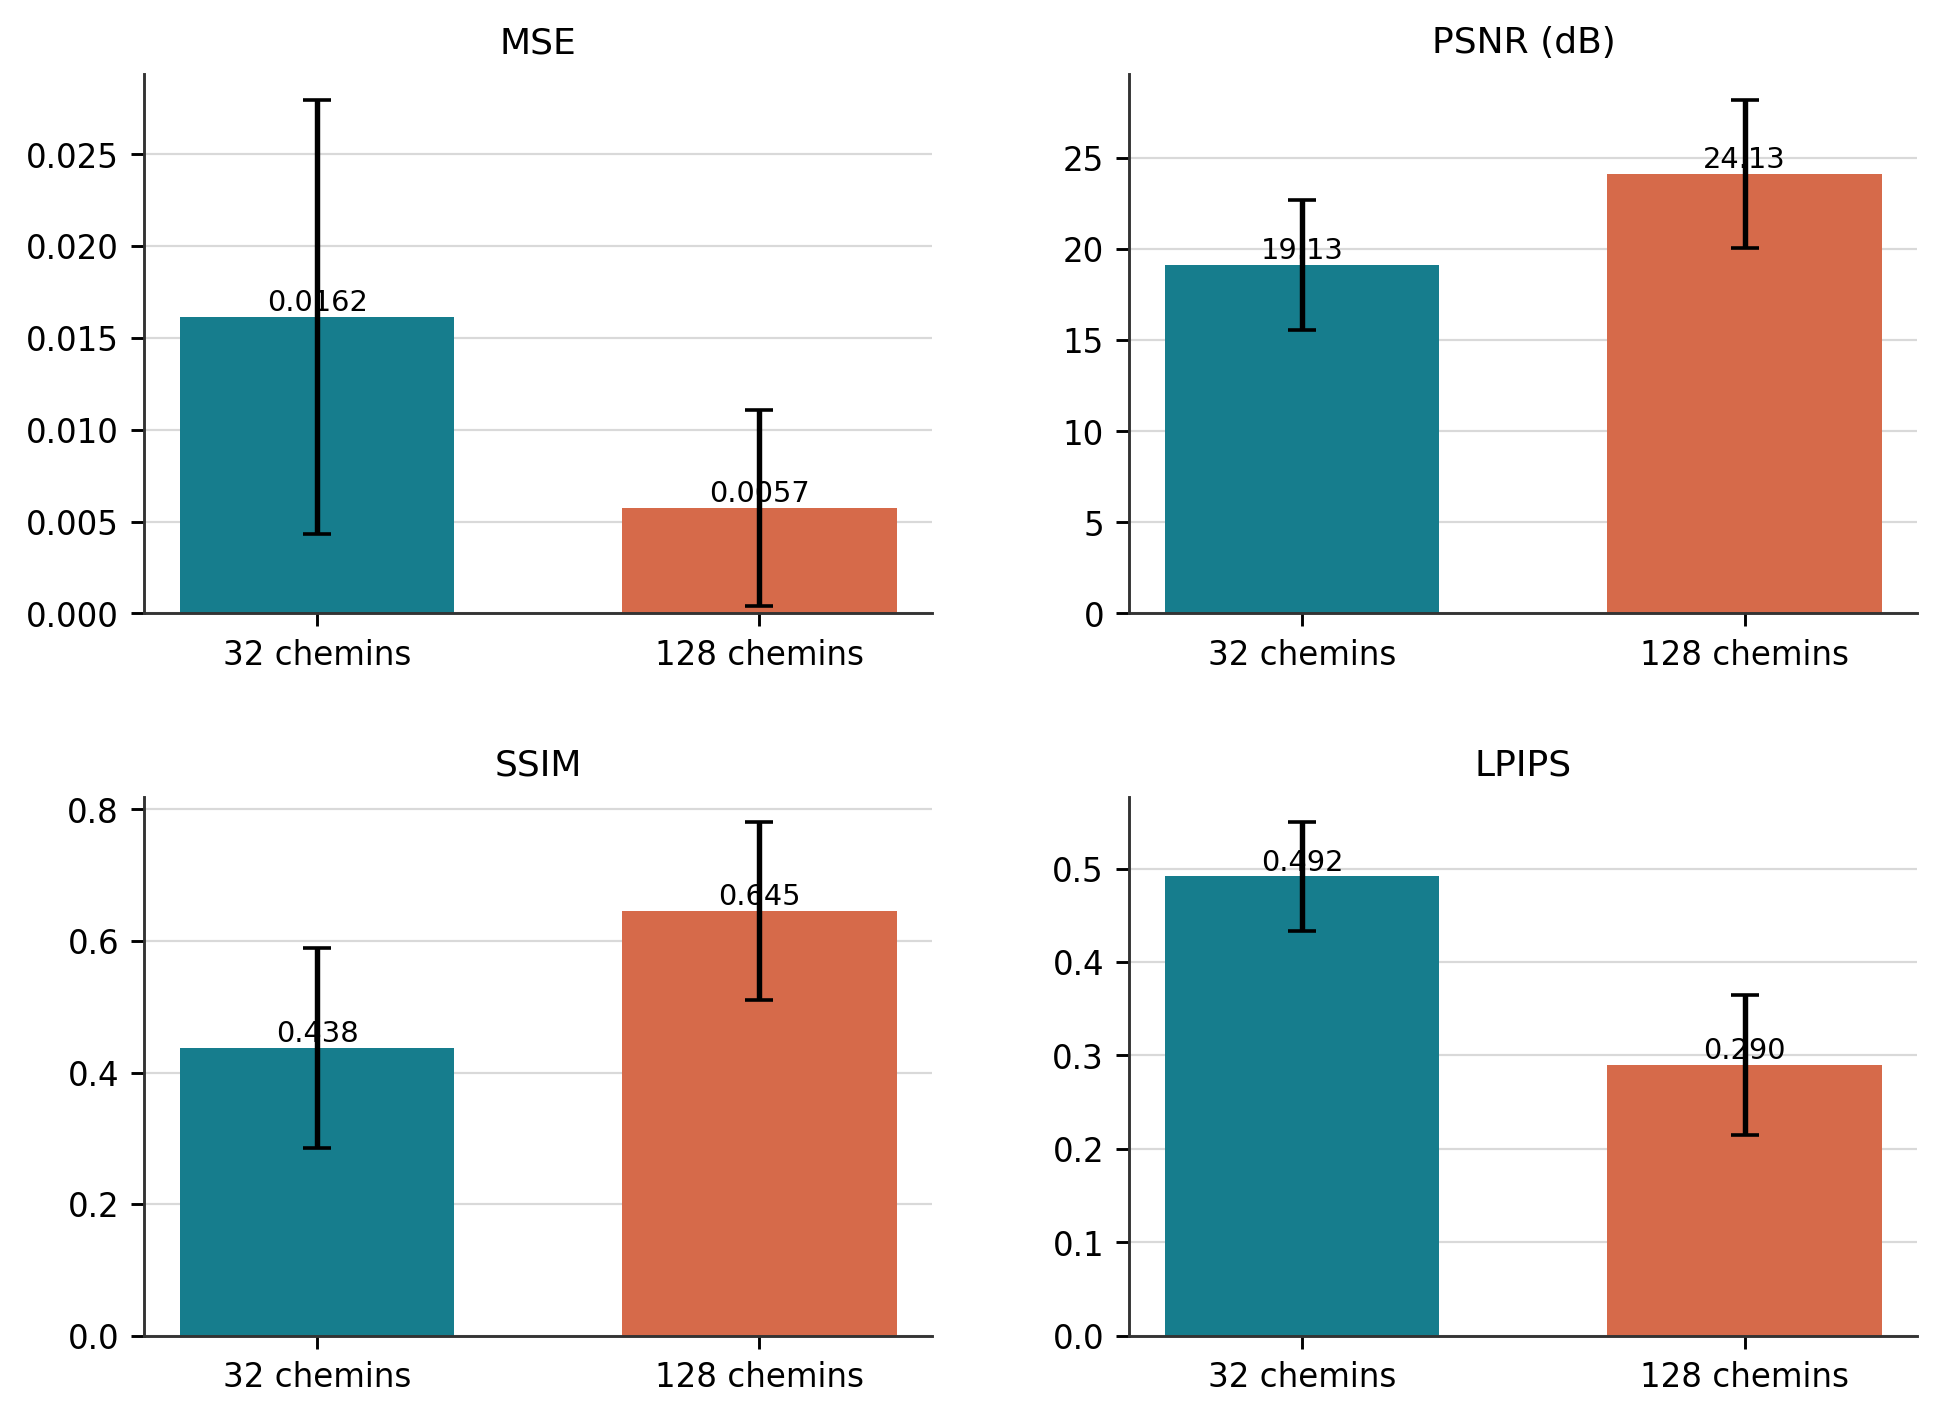
\includegraphics[width=\linewidth,height=6.15cm,keepaspectratio]{ch3_comparaison_quantitative.png}
    \end{column}
    \begin{column}{0.29\textwidth}
      \begin{block}{Configuration 128}
        \begin{itemize}\small
          \item MSE : $0{,}00573$;
          \item PSNR : $24{,}13$ dB;
          \item SSIM : $0{,}645$;
          \item LPIPS : $0{,}290$.
        \end{itemize}
      \end{block}

      \begin{alertblock}{Compromis}
        Meilleure reconstruction, mais environ 4 fois plus de chemins et un temps total multiplié par $2{,}67$.
      \end{alertblock}
    \end{column}
  \end{columns}
  \source{Les budgets d'entraînement diffèrent; cette comparaison n'isole pas l'effet causal du nombre de chemins.}
\end{frame}

\begin{frame}{Effet visuel du budget de chemins}
  \centering
  \begin{tikzpicture}
    \clip (0,0) rectangle (\textwidth,4.65cm);
    \node[anchor=north west,inner sep=0] at (0,4.65cm)
      {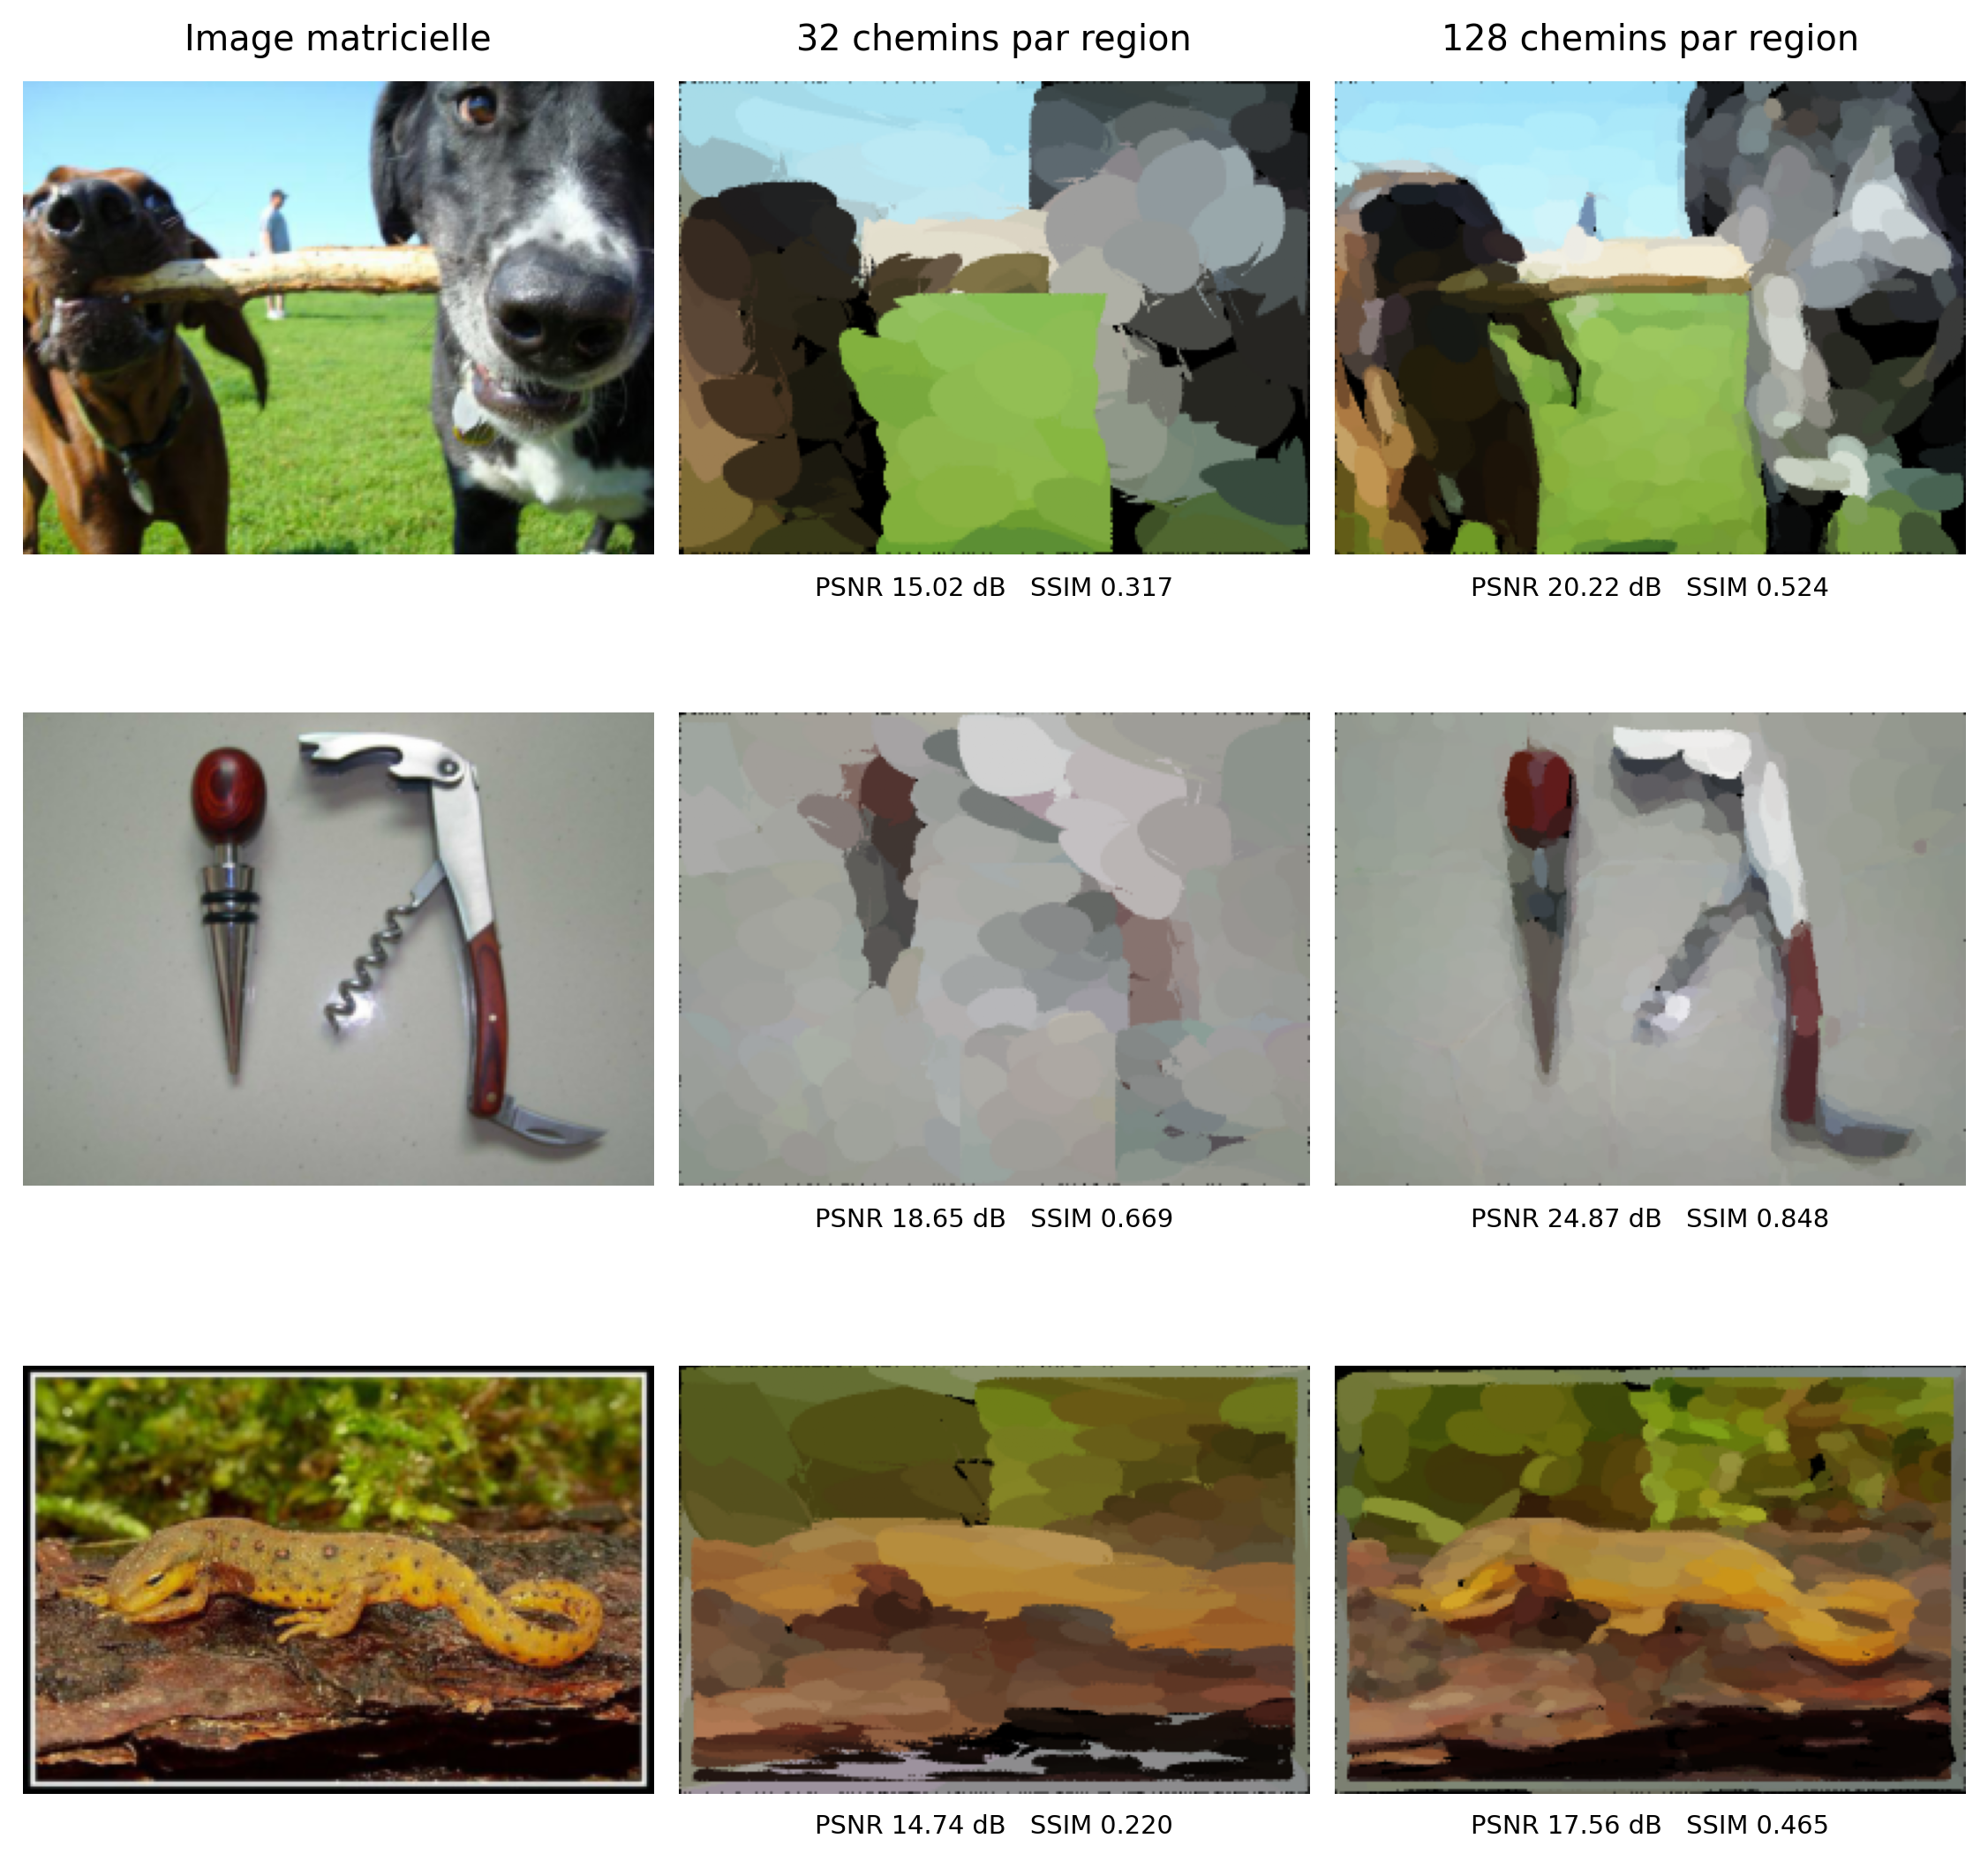
\includegraphics[width=\textwidth]{ch3_comparaison_qualitative.png}};
  \end{tikzpicture}

  \vspace{0.25cm}
  \begin{columns}[T,onlytextwidth]
    \begin{column}{0.32\textwidth}
      \metric{PSNR}{$15{,}02\rightarrow20{,}22$ dB}{Blue}
    \end{column}
    \begin{column}{0.32\textwidth}
      \metric{SSIM}{$0{,}317\rightarrow0{,}524$}{Teal}
    \end{column}
    \begin{column}{0.32\textwidth}
      \metric{Observation}{Détails plus reconnaissables}{Coral}
    \end{column}
  \end{columns}

  \source{L'image reste stylisée : les aplats de couleur remplacent les textures photographiques fines.}
\end{frame}

\begin{frame}{Comparaison externe : fidélité}
  \begin{columns}[T,onlytextwidth]
    \begin{column}{0.72\textwidth}
      \centering
      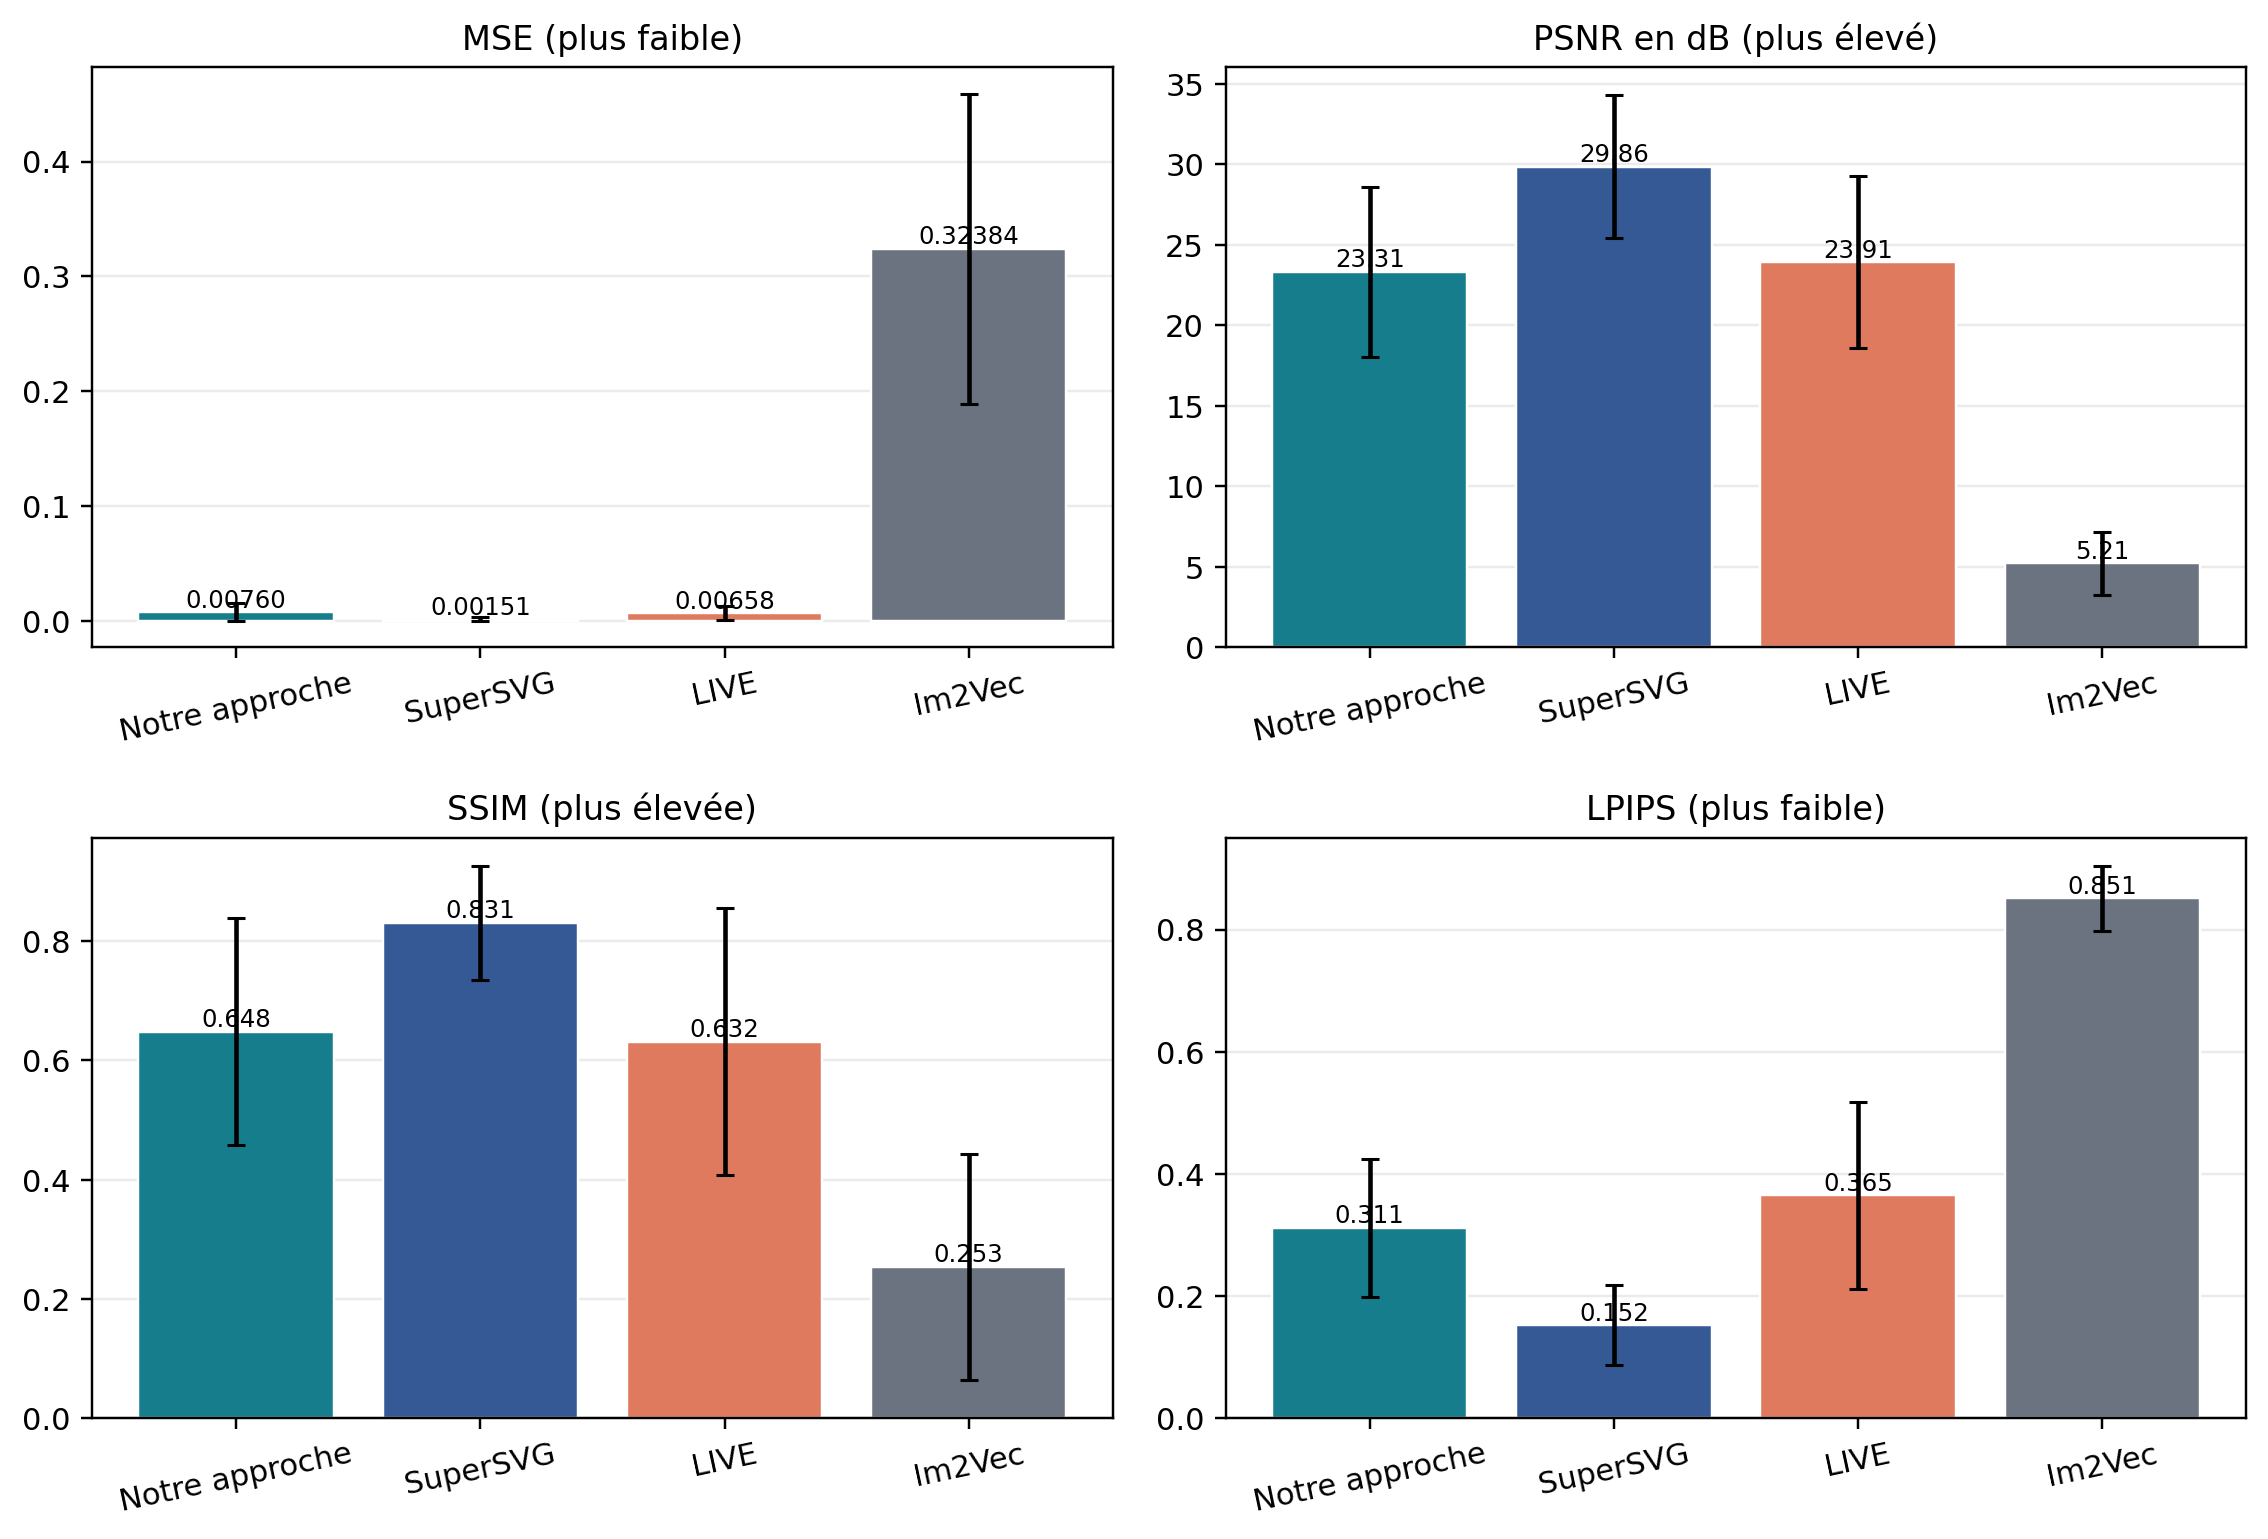
\includegraphics[width=\linewidth,height=6.15cm,keepaspectratio]{ch3_comparaison_methodes_quantitative.png}
    \end{column}
    \begin{column}{0.24\textwidth}
      \begin{block}{SuperSVG}
        Meilleure moyenne pour les quatre métriques.
      \end{block}
      \begin{block}{Notre approche}
        Proche de LIVE; meilleure SSIM et LPIPS moyennes.
      \end{block}
      \begin{alertblock}{Im2Vec}
        Checkpoint emoji évalué hors domaine; résultats non exploitables sur ces photographies.
      \end{alertblock}
    \end{column}
  \end{columns}
  \source{Moyennes et écarts-types calculés sur quatre images communes.}
\end{frame}

\begin{frame}{Comparaison externe : résultats visuels}
  \centering
  \begin{tikzpicture}
    \clip (0,0) rectangle (0.88\textwidth,5.15cm);
    \node[anchor=north west,inner sep=0] at (0,5.15cm)
      {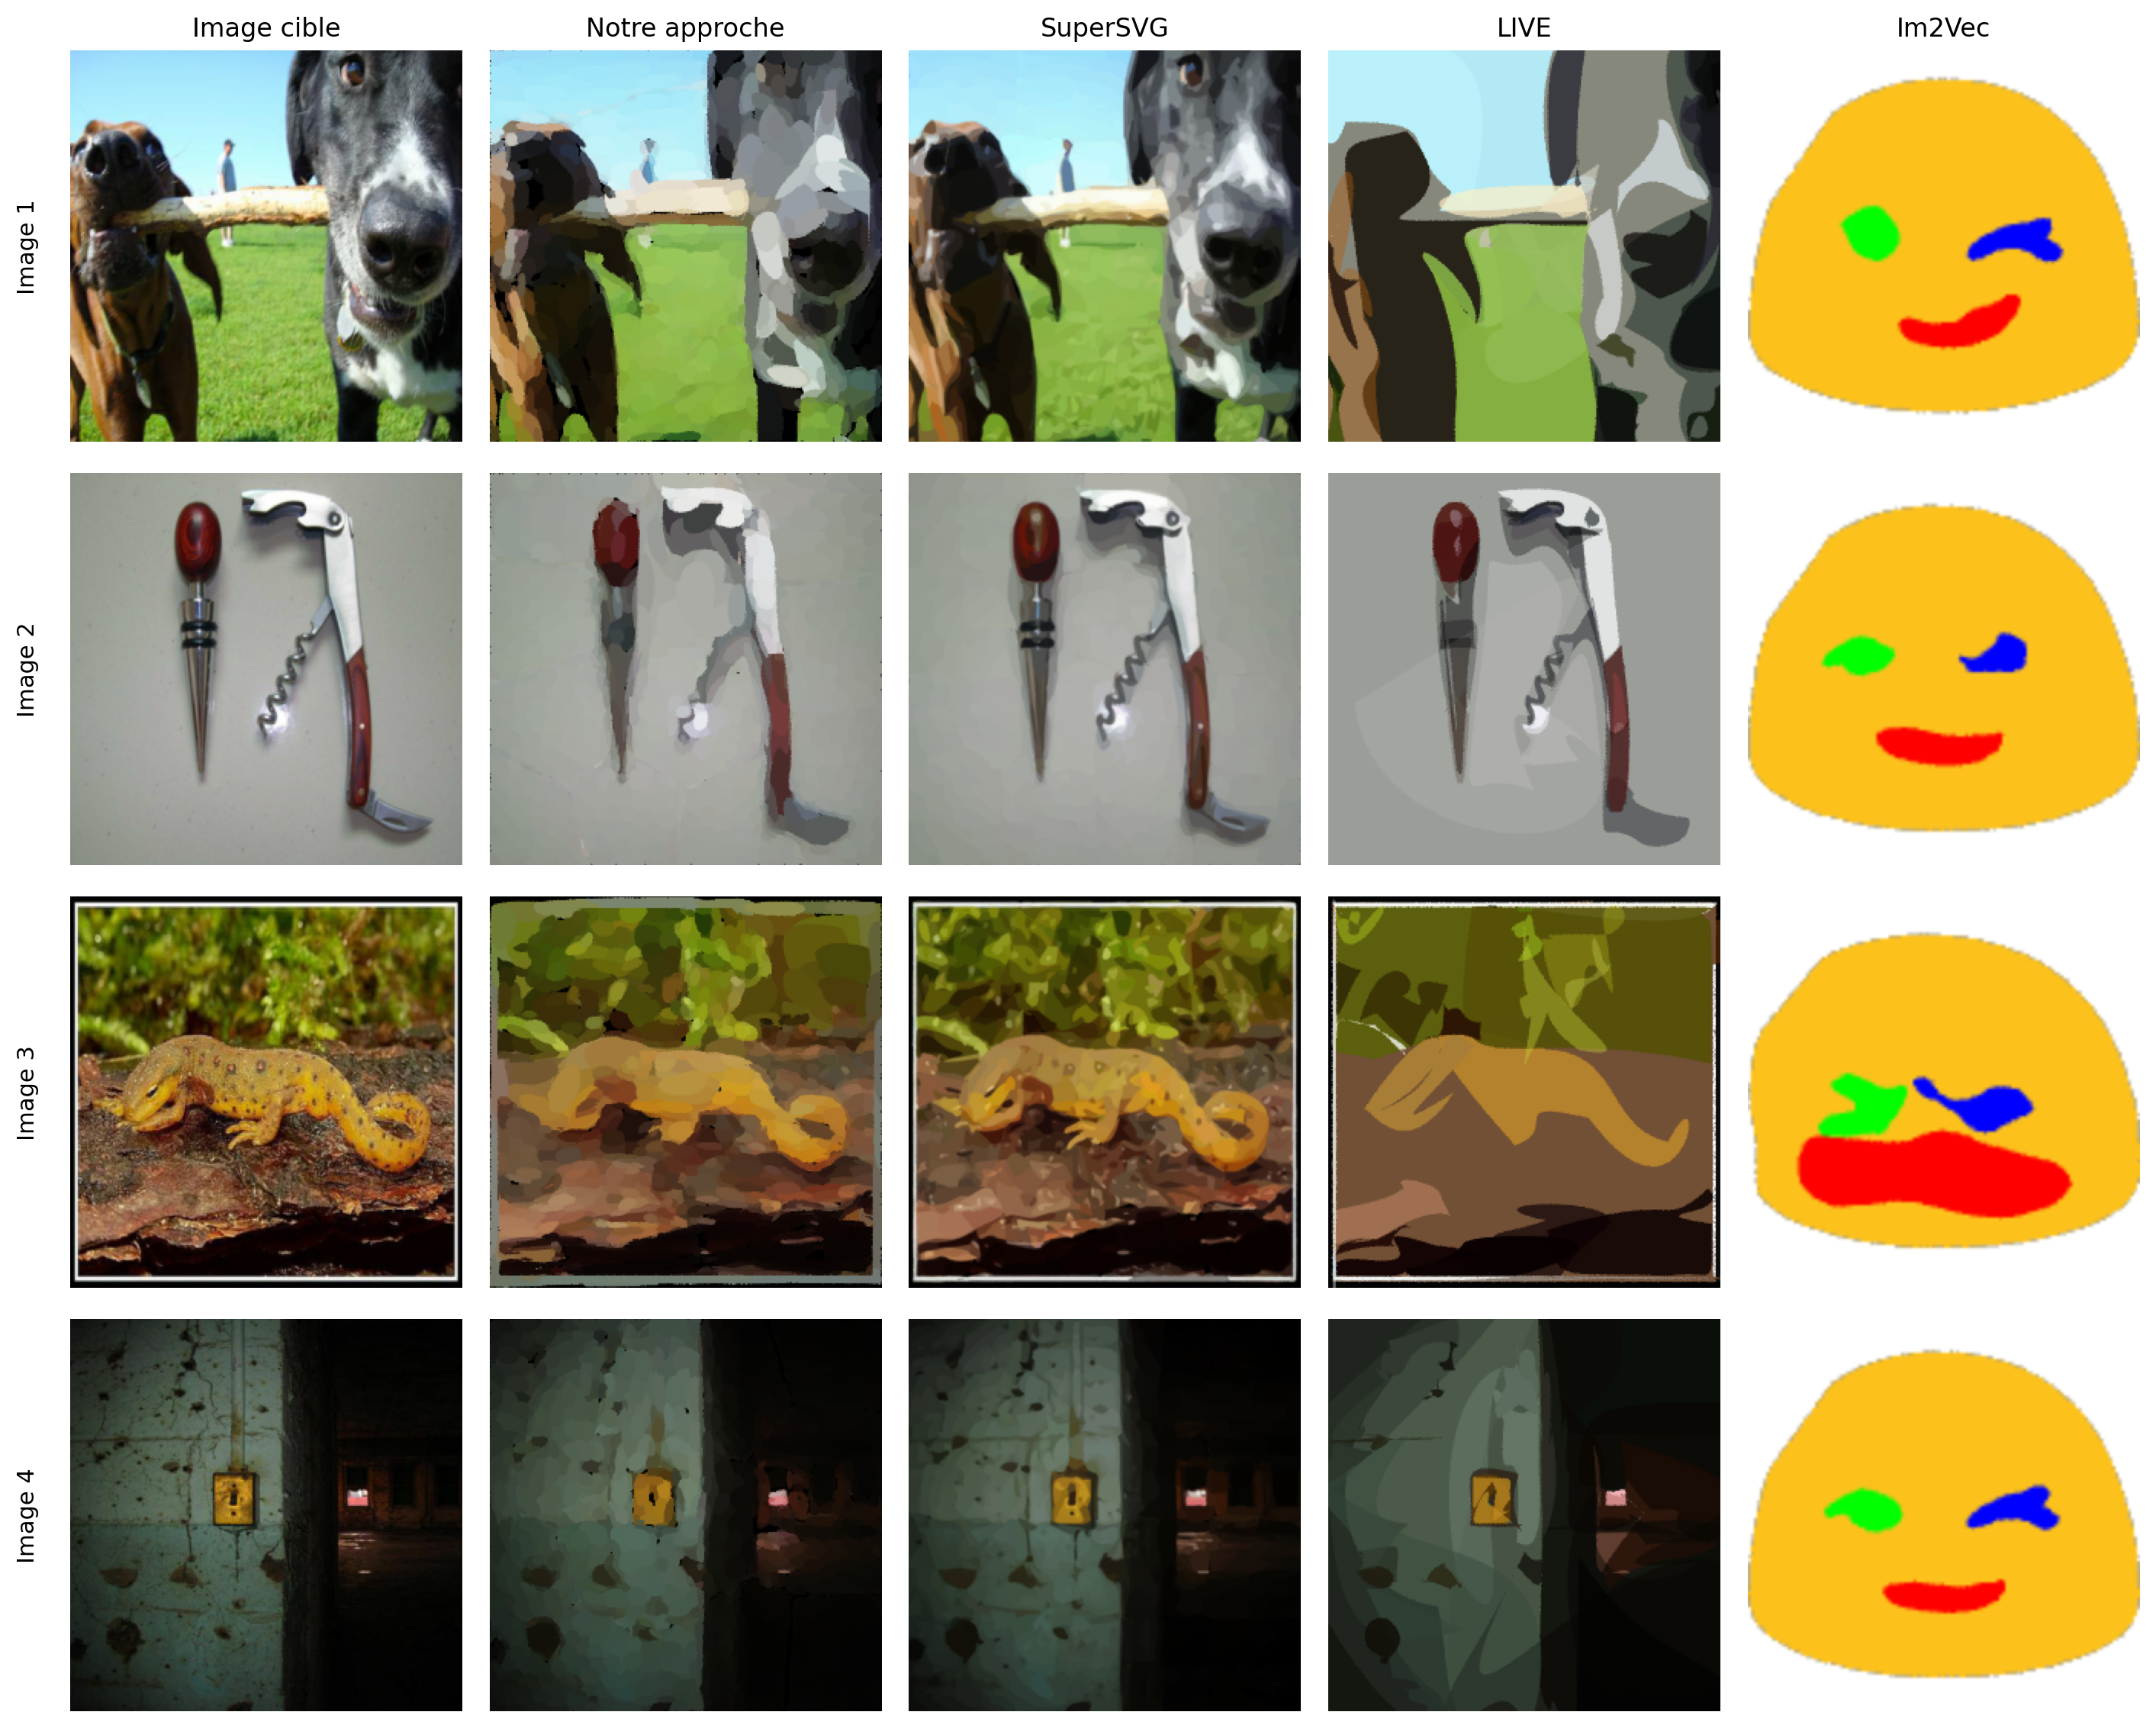
\includegraphics[width=0.88\textwidth]{ch3_comparaison_methodes_qualitative.png}};
  \end{tikzpicture}

  \vspace{0.2cm}
  \begin{columns}[T,onlytextwidth]
    \begin{column}{0.32\textwidth}
      \centering\small\bfseries\color{Teal}Notre approche\par
      \scriptsize Formes principales et couleurs dominantes conservées.
    \end{column}
    \begin{column}{0.32\textwidth}
      \centering\small\bfseries\color{Blue}SuperSVG\par
      \scriptsize Détails et structures les plus proches de la cible.
    \end{column}
    \begin{column}{0.32\textwidth}
      \centering\small\bfseries\color{Coral}LIVE\par
      \scriptsize Simplification plus marquée avec seulement 32 chemins.
    \end{column}
  \end{columns}
\end{frame}

\begin{frame}{Compromis qualité, temps et complexité}
  \centering
  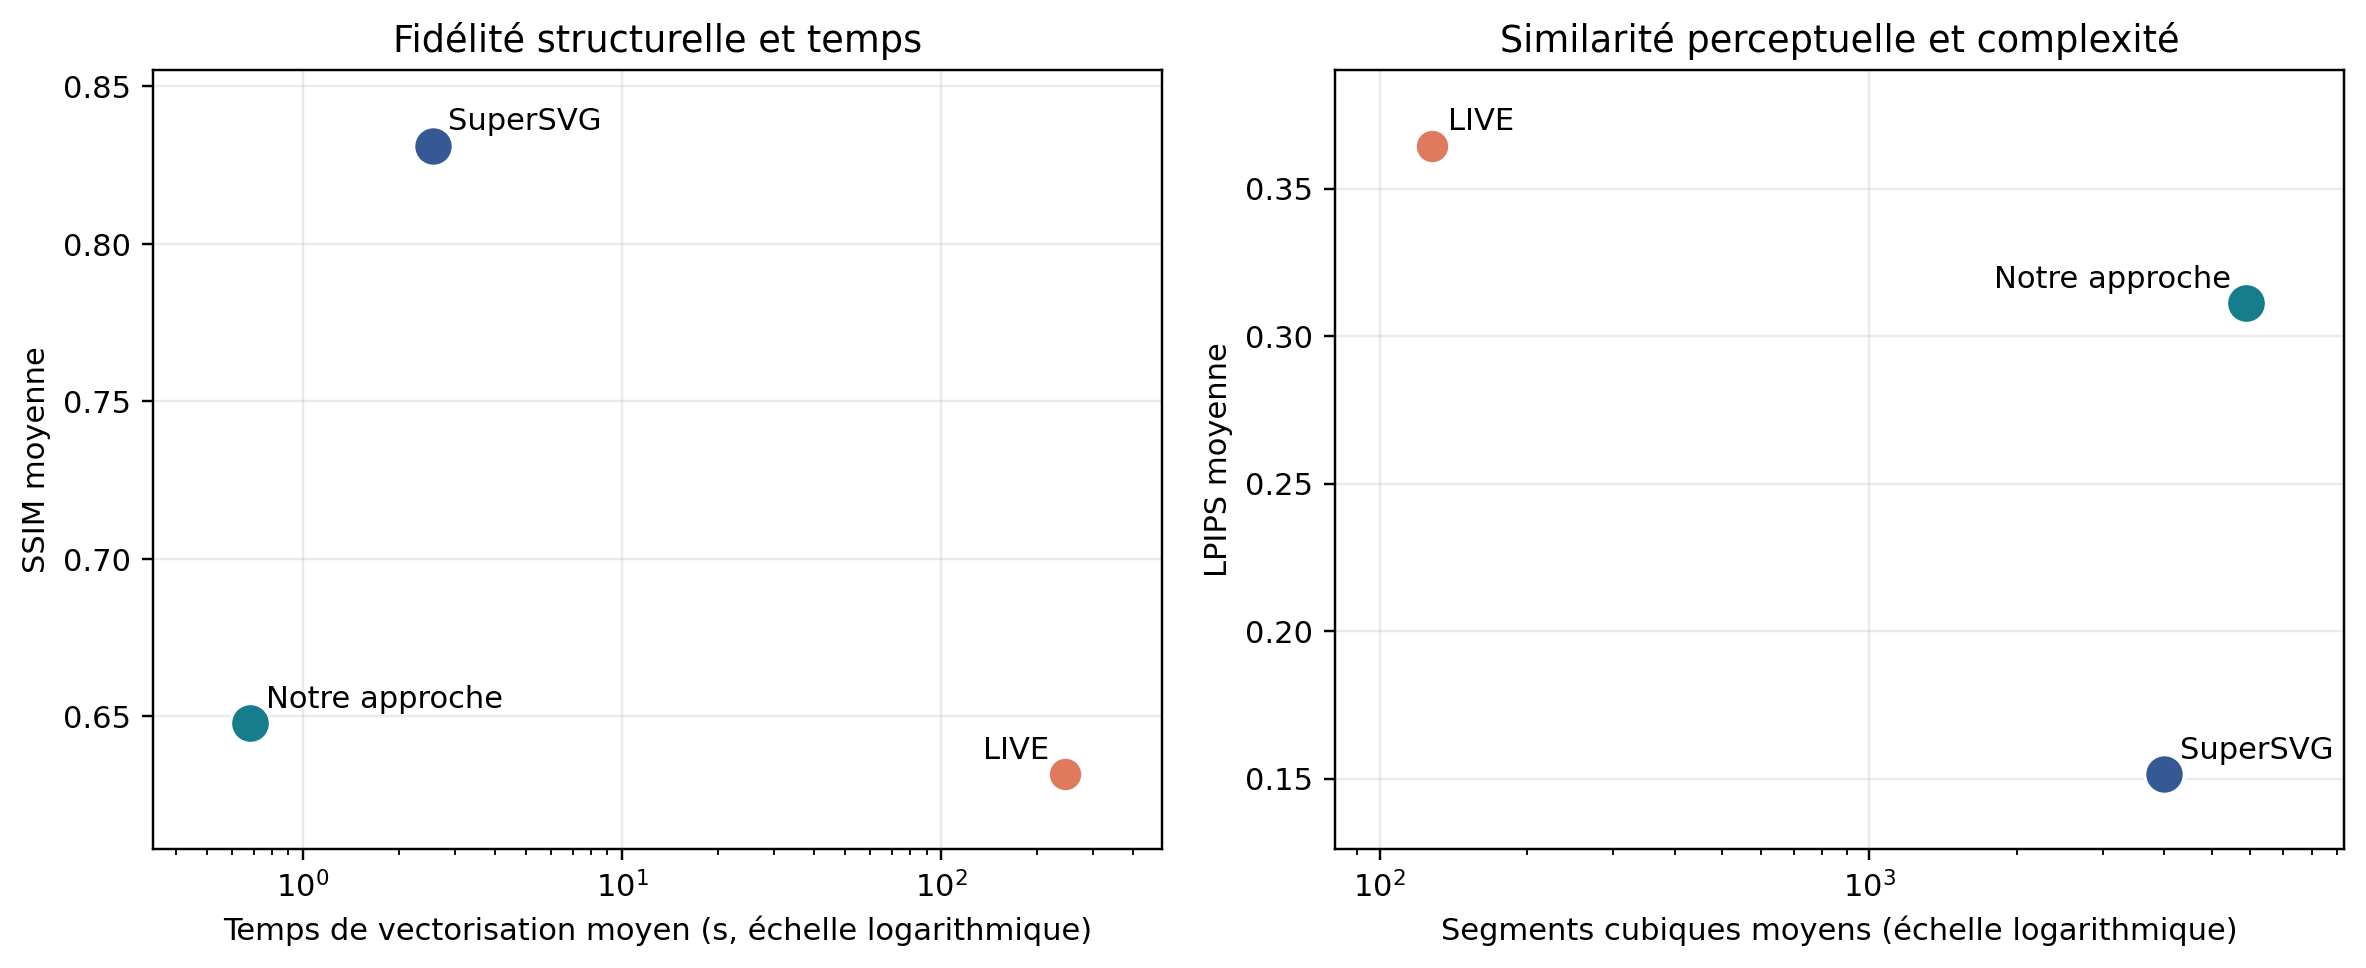
\includegraphics[width=0.96\textwidth]{ch3_compromis_methodes.png}

  \vspace{0.15cm}
  \begin{columns}[T,onlytextwidth]
    \begin{column}{0.32\textwidth}
      \metric{Notre approche}{$0{,}684$ s · $1\,472$ chemins}{Teal}
    \end{column}
    \begin{column}{0.32\textwidth}
      \metric{SuperSVG}{$2{,}548$ s · $1\,000$ chemins}{Blue}
    \end{column}
    \begin{column}{0.32\textwidth}
      \metric{LIVE}{$243{,}804$ s · $32$ chemins}{Coral}
    \end{column}
  \end{columns}

  \source{Im2Vec est exclu de l'analyse temporelle : ses quatre chemins ne reconstruisent pas le contenu du benchmark.}
\end{frame}

% -----------------------------------------------------------------------------
\section{Limites et conclusion}
% -----------------------------------------------------------------------------

\begin{frame}{Limites et perspectives}
  \begin{columns}[T,onlytextwidth]
    \begin{column}{0.48\textwidth}
      \begin{alertblock}{Limites actuelles}
        \begin{itemize}
          \item nombre fixe de chemins par superpixel;
          \item régions prédites indépendamment;
          \item formes uniquement fermées, opaques et remplies;
          \item SVG volumineux et difficiles à éditer;
          \item benchmark réduit et configurations hétérogènes.
        \end{itemize}
      \end{alertblock}
    \end{column}
    \begin{column}{0.48\textwidth}
      \begin{block}{Perspectives}
        \begin{itemize}
          \item prédire la présence ou l'arrêt des chemins;
          \item supprimer et fusionner les primitives redondantes;
          \item ajouter un raffinement global \textit{coarse-to-fine};
          \item intégrer des pertes perceptuelles et structurelles;
          \item étendre le benchmark avec des budgets contrôlés.
        \end{itemize}
      \end{block}
    \end{column}
  \end{columns}

  \vfill
  \takeaway{Objectif futur : conserver la vitesse de la prédiction directe tout en rapprochant la fidélité de SuperSVG et la compacité de LIVE.}
\end{frame}

\begin{frame}{Conclusion}
  \vspace{0.2cm}
  \begin{enumerate}
    \item \textbf{Une chaîne complète raster-vers-SVG}\par
      SLIC, DINOv3, attention, courbes de Bézier et export vectoriel dans un même système.
      \vspace{0.35cm}
    \item \textbf{Un apprentissage sans vérité terrain vectorielle}\par
      DiffVG permet de superviser les coordonnées et les couleurs directement depuis les pixels.
      \vspace{0.35cm}
    \item \textbf{Un compromis expérimental clairement identifié}\par
      Notre approche est rapide et produit des SVG valides, mais doit encore gagner en fidélité et en compacité.
  \end{enumerate}

  \vfill
  \takeaway{Le projet fournit une base fonctionnelle pour une vectorisation plus adaptative, plus compacte et mieux raccordée à l'échelle globale.}
\end{frame}

\begin{frame}[plain]
  \begin{tikzpicture}[remember picture,overlay]
    \fill[Ink] (current page.south west) rectangle (current page.north east);
    \fill[Teal] (current page.south west) rectangle
      ([xshift=0.16cm]current page.north west);
    \node[anchor=north,fill=white,rounded corners=2pt,inner sep=0.12cm]
      at ([yshift=-0.75cm]current page.north)
      {
\includegraphics[height=1.65cm]{his_logo.png}};
    \node[text=white,font=\bfseries\fontsize{29}{34}\selectfont]
      at ([yshift=0.25cm]current page.center) {Merci pour votre attention};
    \node[text=white!72,font=\Large]
      at ([yshift=-0.75cm]current page.center) {Questions et discussion};
    \node[text=Coral,font=\large\bfseries]
      at ([yshift=1.05cm]current page.south) {Amir BITAM · Zakaria AITHAMOUDI};
  \end{tikzpicture}
\end{frame}

\end{document}
